%\begin{savequote}[8cm]
%  ``Those who can, do; those who can't, teach.''
%  \qauthor{Dan Zevin}
%\end{savequote}
%\makeatletter
\chapter{Applications}
\label{Applications}

\section{Fast Summation of radial Functions on the Sphere}
\label{Applications:FastSum}
\emph{Radial basis functions} are a powerful tool in many areas of multi-dimensional 
approximation and interpolation, in particular for scattered data. Other applications
are the numerical solution of partial differential equations and artificial neural networks 
for nonparametric regression.
In radial basis function methods one approximates a function $g: \R^n
\rightarrow \R$, $n \in \N$, by a linear combination $f$ of the form
\begin{equation}
  \nonumber
  %\label{Applications:RBFSum}
  \fun{f}{\V{x}} := \sum_{l=0}^L b_{l} \fun{\phi}{\norm{\V{y}_{l}-\V{x}}},
\end{equation}
where $\V{x}, \V{y}_{l} \in \R^n$, $b_{l} \in \R$ for $L \in \N$, and 
$\phi: \Rp \rightarrow \R$ is a function on the positive real line. 
The functions $\set{\fun{\phi}{\norm{\V{y}-\cdot}}}_{l=0}^{L-1}$ are
denoted \emph{radial basis functions} since they depend solely on 
the distance of the argument $\V{x}$ to a fixed point $\V{y}_{l}$ measured 
by a suitable norm $\norm{\cdot}$, which is usually intended to be euclidean.
Moreover, these functions are in loosely speaking \emph{localizing} in the sense 
that they rapidely outside a neighbourhood of $\V{y}_{l}$.

The spherical counterpart of radial basis function are the \emph{spherical radial basis functions} or \emph{zonal} functions as introduced in section 
\ref{Basics:SphericalKernels}. The norm $\norm{\cdot}$ is replaced by the usual
inner product $\scalarproduct{\cdot}{\cdot}_{\Ln{2}{\twosphere}}$, i.e. one
approximates a function $g: \twosphere \rightarrow \R$ by
\begin{equation}
  \label{Applications:ZonalSum}
  \fun{f}{\V{\xi}} := \sum_{l=0}^L b_{l} \fun{K}{\V{\eta}_{l}\cdot\V{\xi}}.
\end{equation}
with $\V{\xi}, \V{\eta}_{l} \in \twosphere$, $b_{l} \in \R$ for $L \in \N$, and 
$K: [-1,1] \rightarrow \R$ is now a function on the closed interval $[-1,1]$. 
The fact that the geodesic distance of two points $\V{\xi}$ and $\V{\eta}$ on the 
sphere $\twosphere$ is $\sqrt{2-2\V{\xi}\cdot\V{\eta}}$ justifies the choice.

An essential task is the fast evaluation such linear combinations. More formally, 
one wants to evaluate the sum \eqref{Applications:ZonalSum}
on a set of \emph{target nodes} 
$$
  \mathcal{X} := \pset{\V{\xi}_{d} \in \twosphere}{|}{d=0,\ldots,D-1,\ D \in \N}
$$ 
with 
$$
  \mathcal{Y} := \pset{\V{\eta}_{l} \in \twosphere}{|}{l = 0,\ldots,L-1,\ L \in \N}
$$
being the denoted the set of \emph{source nodes}.

Clearly, the construction of fast algorithms for this task depends strongly on the
choice of the function $K$, and conditions imposed on the distribution of the 
source and target nodes, $\mathcal{Y}$ and $\mathcal{X}$, respectively.
If, for example, these sets of nodes are fixed for all evaluations, one might 
precompute all values $ \fun{K}{\V{\eta}_{l}\cdot\V{\xi}_{d}}$ for $l=0,\ldots,L-1$ and 
$d=0,\ldots,D-1$.
The naive approach, i.e. evaluating \eqref{Applications:ZonalSum} for every $\V{\xi}_{d} \in \mathcal{X}$ clearly leads to an $\bigo{L\:D}$ algorithm. For large $L$ and $D$ the computational effort becomes quickly unaffordable.
Quite effective algorithms are often derived by only approximating the desired result 
up an adjustable accuracy. In this case, the localizing property of the function $K$ 
generally has a strong impact. If the function $K$ localizes well and the source nodes 
are not clustered too much, one might take for the evaluation of $f$ at a single target node $\V{\xi}_{d}$ only those functions $\fun{K}{\V{\eta}_{l}\:\cdot}$ into consideration, for
which $\V{\eta}_{l}$ lies in a certain neighborhood of $\V{\xi}_{d}$. This corresponds to truncating the support of the function $K$. If $K$ is already finitely supported this even
yields exact algorithms. 
The \emph{panel clustering} method introduced in \cite{FrGlSch98} reduces the computational effort to evaluate \eqref{Applications:ZonalSum} based on the traditional method of dividing the evaluation od \eqref{Applications:ZonalSum} into near- and far-field. For every function
$\fun{K}{\V{\eta} \: \cdot}$, the near-field contribution is calculated exactly whereas the contribution of the far-field may be approximated coarsely due to the supposed rapid decay of $\fun{K}{\V{\eta} \: \cdot}$. 

Instead of the truncation idea from above, which can be interpreted as a truncation in ''\emph{space}'', we propose a truncation in ''\emph{frequency}'' referring to the
$\Ln{2}{\twosphere}$ basis $\set{Y_{k}^n}_{k\in\NZ; n = -k,\ldots,k}$ of spherical 
harmonics. The Addition Theorem \ref{Basics:AdditionTheorem} provides a 
representation of the function $K$ that separates source and target nodes and 
therefore allows for the construction of fast algorithms. The connection is as 
follows: Using the representation \eqref{Basics:Kernel}, we obtain
\begin{equation}
  \label{Applications:KSeries}
  \fun{K}{\V{\eta}_{l} \cdot \V{\xi}} = \sum_{k=0}^{\infty} \sum_{n=-k}^k 
  \fun{K^{\wedge}}{k}   \fun{Y_{k}^n}{\V{\xi}} \overline{\fun{Y_{k}^n}{\V{\eta}_{l}}}
\end{equation}
where we recall the Legendre transform $K^{\wedge}$of $K$
\[
  \fun{K^{\wedge}}{k} := 2 \pi \int_{-1}^{1} \fun{K}{x} \fun{P_{k}}{x} \dx x 
  \quad \paren{k \in \NZ}.
\]
Now, truncating at a fixed index $M \in \NZ$, i.e.
\begin{equation}
  \label{Applications:TruncatedSeries}
  \fun{K_{M}}{\V{\eta}_{l} \cdot \V{\xi}} := 
  \sum_{k=0}^{M} \sum_{n=-k}^k \fun{K^{\wedge}}{k} \fun{Y_{k}^n}{\V{\xi}} \overline{\fun{Y_{k}^n}{\V{\eta}_{l}}}
\end{equation}
we approximate $f$ by $f_{M}$ with
\begin{equation}
  \nonumber
  \begin{split}
    \fun{f}{\xi} \approx \fun{f_{M}}{\xi} & := \sum_{l = 0}^{L-1} b_{l} \fun{K_{M}}{\V{\eta}_{l} \cdot \V{\xi}} \\
                 &       = \sum_{l = 0}^{L-1} b_{l} \sum_{k=0}^{M} \sum_{n=-k}^k \fun{K^{\wedge}}{k}
                           \fun{Y_{k}^n}{\V{\xi}} \overline{\fun{Y_{k}^n}{\V{\eta}_{l}}} \\
                 &       = \sum_{k=0}^{M} \sum_{n=-k}^k \paren{\sum_{l = 0}^{L-1} b_{l}
                           \overline{\fun{Y_{k}^n}{\V{\eta}_{l}}}} \fun{K^{\wedge}}{k} \fun{Y_{k}^n}{\V{\xi}}.
  \end{split}                           
\end{equation}
The sums
\begin{equation}
\label{Applications:AdjointNDSFT}
  \tilde{b}_{k}^n := \sum_{l = 0}^{L-1} b_{l} \overline{\fun{Y_{k}^n}{\V{\eta}_{l}}} \quad \paren{(k,n) \in \mathcal{I}^M}
\end{equation}
can be evaluated by the adjoint NFSFT algorithm (see Algorithm 
\ref{NFSFT:Algorithm:adjointNFSFT}) and we arrive at
\[
  \fun{f_{M}}{\xi} = \sum_{k=0}^{M} \sum_{n=-k}^k \tilde{b}_{k}^n \fun{K^{\wedge}}{k}
                     \fun{Y_{k}^n}{\V{\xi}} = \sum_{k=0}^{M} \sum_{n=-k}^k a_{k}^n
                     \fun{Y_{k}^n}{\V{\xi}},
\]
where we let $a_{k}^n := \tilde{b}_{k}^n \fun{K^{\wedge}}{k}$. Finally, the evaluation of
\begin{equation}
\label{Applications:NDSFT}
  \fun{f_{M}}{\V{\xi}} = \sum_{k=0}^{M} \sum_{n=-k}^k a_{k}^n \fun{Y_{k}^n}{\V{\xi}}
\end{equation}
on the set of target nodes $\mathcal{X}$ can be carried out by the NFSFT algorithm 
(cf. Algorithm \ref{NFSFT:Algorithm:NFSFT}). The NFSFT algorithms have complexity 
$\bigo{M^3 \log M + L \log \frac{1}{\varepsilon}}$ and 
$\bigo{M^3 \log M + L \log \frac{1}{\varepsilon}}$, respectively. The intermediate 
step consists in computing the coefficients $a_{k}^n$ by $\bigo{M^2}$ multiplications
with the symbol $\fun{K^{\wedge}}{k}$. Since the $M$ is fixed, we have in total an
$\bigo{L + D}$ algorithm the evaluation of $f_{M}$ on $\mathcal{X}$. In particular, the
performance does not depend on the distribution of the source and target nodes, 
$\V{\eta}_{l}$ and $\V{\xi}_{d}$. We summarize this procedure in Algorithm 
\ref{Applications:Algorithm:FastSummation}.

\begin{remark}
  The proposed algorithm is approximative in multiple ways. First, the systematic 
  error introduced by truncating the series \eqref{Applications:KSeries} at the 
  index $M$ limits the 
  achievable accuracy. Moreover, the NFSFT algorithm and its adjoint 
  are approximative themselves. First, the FLFT part is limited by the choice of the
  threshold during precomputation. Second, the invocation of the NFFT and adjoint 
  NFFT algorithms introduces an error, since these algorithms are by definition yet
  approximative. In total, one has to adjust the corresponding parameters accordingly 
  to yield an accurate result.
  However, replacing the NFSFT and adjoint NFSFT by its direct versions called NDSFT and 
  adjoint NDSFT still yields an $\bigo{L + D}$. Under the assumption that these are 
  stable, $M$ remains the only accuracy-limiting parameter.
\end{remark}

\begin{remark}
  Algorithm \ref{Applications:Algorithm:FastSummation} also admits complex 
  coefficients $b_{l} \in \C$. This gives rise to generally complex valued 
  linear combinations $f$. Moreover, we could also permit complex-valued 
  symbol coefficients $\fun{K^{\wedge}}{k,n} \in \C$ that even depend on $n$. 
\end{remark}

\begin{remark}
	The whole algorithm can be expressed in matrix-vector notation. This reads
	\[
	  \V{f}_{\mathcal{X}} = \V{Y}_{\mathcal{X}} \: \V{W} \:
	  \V{Y}_{\mathcal{Y}}^{\h} \: \V{b}
	\]
	with
	\begin{align}
	  \nonumber
	  \V{f}_{\mathcal{X}} & := \paren{\fun{f_{M}}{\V{\xi}_{d}}}_{d=0}^{D-1} \in \R^D,\\
	  \nonumber
	  \V{Y}_{\mathcal{X}} & := \paren{\fun{Y_k^n}{\V{\xi}_{d}}}_{d=0,\ldots,D-1; 
	  \paren{k,n} \in \mathcal{I}^M} \in \C^{D \times \paren{M+1}^2}. \\
	  \nonumber
	  \V{W} & := \fun{\diag}{\V{w}},\ \V{w} := \paren{w_{k}^n}_{\paren{k,n} \in 
	  \mathcal{I}^M} \in \R^{(M+1)^2},\ w_{k}^n := \fun{K^{\wedge}}{k}, \\
	  \nonumber
	  \V{Y}_{\mathcal{Y}} & := \paren{\fun{Y_k^n}{\V{\eta}_{l}}}_{l=0,\ldots,L-1;
	  \paren{k,n} \in \mathcal{I}^M} \in \C^{L \times \paren{M+1}^2}
	\end{align}
\end{remark}

\begin{algorithm}[tb]
  \caption{Fast Summation}
  \label{Applications:Algorithm:FastSummation}    
  \begin{algorithmic}
    \STATE  Input:  $L \in \N$, $\paren{b_{l}}_{l=0}^{L-1}$, 
    $\paren{\V{\eta}_{l}}_{l=0}^{L-1}$, $D \in \N$, 
    $\paren{\V{\xi}_{d}}_{d=0}^{D-1}$, $M \in \NZ, 
    \paren{\fun{K^{\wedge}}{k}}_{k=0}^M$
    \STATE
    \STATE Compute $\paren{\tilde{b}_{k}^n}_{\paren{k,n} \in \mathcal{I}^M}$ 
    by a fast adjoint NFSFT
    \STATE 
    \FOR {$k=0,\ldots,M$} 
      \FOR {$n=-k,\ldots,k$} 
        \STATE $a_{k}^n := \tilde{b}_{k}^n \fun{K^{\wedge}}{k}$
      \ENDFOR
    \ENDFOR
    \STATE
    \STATE Compute $\paren{\fun{f}{\V{\xi}_{d}}}_{d=0}^{D-1}$ by a fast NFSFT
    \STATE
    \STATE Output: $\paren{\fun{f}{\V{\xi}_{d}}}_{d=0}^{D-1}$
\end{algorithmic}
\end{algorithm}

\subsection{Error estimates}

\begin{lemma}\label{lemma:error}
  The proposed approximation obeys the uniform error estimate
  \begin{equation}
    \label{Applications:UniformErrorBound}
    \left\|\V{f} - \V{f}_{M}\right\|_{\infty} \le \left\|\V{b}\right\|_1 \sum_{k>M}
    \frac{2k+1}{4\pi} \abs{\fun{K^{\wedge}}{k}}.
  \end{equation}
\end{lemma}
\begin{proof}
  We obtain immediately
  \begin{align*}
    \left\|\V{f} - \V{f}_{M}\right\|_{\infty} 
    & = \max_{\V{\xi} \in \mathcal{X}} 
        \left|\sum_{l=0}^{L-1} b_{l} \sum_{k>M} \frac{2k+1}{4\pi} \fun{K^{\wedge}}{k} 
        \fun{P_{k}}{\V{\eta}_{l} \cdot \V{\xi}}\right| \\
    & \le \sum_{l=0}^{L-1} \left| b_{l} \right| \max_{\V{\xi} \in \mathcal{X}} 
      \left| \sum_{k>M} \frac{2k+1}{4\pi} \fun{K^{\wedge}}{k} 
      \fun{P_{k}}{\V{\eta}_{l} \cdot \V{\xi}} \right| \\
    & \le \left\|\V{b}\right\|_1 \sum_{k>M} \frac{2k+1}{4\pi} \abs{\fun{K^{\wedge}}{k}},
  \end{align*}
  where we have used $\left|\fun{P_{k}}{x}\right| \le 1$. 
\end{proof}

For the Poisson kernel \eqref{PoissonKernel} and the singularity kernel
\eqref{SingularityKernel}, we have thereby the following lemma.

\begin{lemma}
 \begin{enumerate}
   \item 
Using the Poisson kernel with $K=Q_h$ within our summation algorithm yields an relative 
error of
     \begin{equation}
       \label{error:poisson}
       \frac{\left\|f - f_{M}\right\|_{\infty}}{\left\|\V{b}\right\|_1} \le
       \frac{h^{M+1}}{4\pi}
       \left(\frac{2M+1}{1-h}+\frac{2}{\left(1-h\right)^2}\right)\, .
     \end{equation}
     \item 
Using the singularity kernel with $K=S_h$ within our summation algorithm yields 
an relative error of
       \begin{equation}
         \label{error:singular}
         \frac{\left\|f - f_{M}\right\|_{\infty}}{\left\|\V{b}\right\|_1} \le
         \frac{h^{M+1}}{4\pi} \left(\frac{2M+1}{2\left(1-h\right)}+
           \frac{4M}{\left(1-h\right)^2}+
         \frac{4}{\left(1-h\right)^3}\right)\, .
       \end{equation}
 \end{enumerate}
\end{lemma}
\begin{proof}
The symbols are given by $\fun{Q_{h}^{\wedge}}{k}=h^k$ and
$\fun{S_{h}^{\wedge}}{k}=\frac{2}{2k+1}h^k$, respectively.
Using Lemma \ref{lemma:error} yields the assertions.
\end{proof}
Simply put, the error decays exponentially with increasing $M$.

The locally supported kernel $L_{h,\lambda}$ also obeys the uniform error bound
\eqref{Applications:UniformErrorBound}. But in contrast to the Poisson kernel 
and Singularity kernel we obtain only a polynomial error decay in $M$.
\begin{lemma}
  For the locally supported kernels $L_{h,\lambda}$ holds:
  \begin{enumerate}
  \item We obtain for fixed $\lambda \in \Rp$ the decay rate
    \[
    \left|\fun{L_{h,\lambda}^{\wedge}}{k}\right| \le C_{\lambda}
    \left(1-h\right)^{-(\lambda+1)}\paren{1-|h|}^{-\frac{1}{4}} 
    k^{-\paren{\floor{\lambda}+\frac{3}{2}}}, 
    \]
where $C_{\lambda}$ is a constant which is independent of $h$ and $k$.
  \item Thus, the relative error of our summation algorithm with this kernel
  is bounded for fixed $\lambda \in \Rp$ by
  \begin{equation}
    \label{error:Lh}
    \frac{\left\|f - f_{M}\right\|_{\infty}}{\left\|\V{b}\right\|_1} \le
    \tilde C_{\lambda} \left(1-h\right)^{-(\lambda+1)}\paren{1-|h|}^{-\frac{1}{4}} 
    M^{-\paren{\floor{\lambda}+\frac{1}{2}}}.
  \end{equation}
where $\tilde C_{\lambda}$ is a constant which is independent of $h$,
$k$ and $M$.
  \end{enumerate}
\end{lemma}

\begin{proof}
  \begin{enumerate}
  \item For $\lambda \in [0,1)$, we have
    \begin{equation*}
      \left|\fun{L_{h,\lambda}^{\wedge}}{k}\right| 
      = \abs{2\pi \int_{h}^1 \frac{\lambda+1}{2\pi\paren{1-h}^{\lambda+1}} 
        \paren{x-h}^{\lambda} \fun{P_{k}}{x} \: \dx x} 
      \le \frac{\lambda+1}{(1-h)^{\lambda+1}}\abs{\int_{h}^1 \fun{P_{k}}{x} \: \dx x}.
    \end{equation*}
    Now, using \eqref{three2} and ${}$ follows
    \begin{align*}
      \frac{\lambda+1}{(1-h)^{\lambda+1}}\abs{\int_{h}^1 \fun{P_{k}}{x} \: \dx x}
      & = \frac{\lambda+1}{(1-h)^{\lambda+1}(2k+1)}
          \abs{\int_{h}^1 \fun{P_{k+1}'}{x} - \fun{P_{k-1}'}{x} \: \dx x}\\
      & = \frac{\lambda+1}{(1-h)^{\lambda+1}(2k+1)}
          \abs{\fun{P_{k-1}}{h} - \fun{P_{k+1}}{h}}\\
      & \le \sqrt{\frac{2}{\pi}}\frac{\lambda+1}{(1-h)^{\lambda+1}(2k+1)
            \sqrt{\sin\arccos h}} \cdot \\
      & \quad \paren{\frac{1}{\sqrt{(k-1)}} + \frac{1}{\sqrt{(k+1)}}},
    \end{align*}
    and with $\sin\arccos h = \sqrt[4]{1-h^2} \ge \sqrt{1-|h|}$ finally
    \begin{equation}
      \label{SmallLambda}
      \left|\fun{L_{h,0}^{\wedge}}{k}\right| \le 
      \sqrt{\frac{2}{\pi}}\frac{\lambda+1}{(1-h)^{\lambda+1}\sqrt{1-|h|}(2k+1)}
      \paren{\frac{1}{\sqrt{(k-1)}} + \frac{1}{\sqrt{(k+1)}}}.
    \end{equation}
    Furthermore, for $\lambda \ge 1$, we obtain by applying \eqref{three2}
    \begin{eqnarray*}
      \left|\fun{L_{h,\lambda}^{\wedge}}{k}\right| &\le&
      \frac{\lambda+1}{\lambda\left(1-h\right)\left(2k+1\right)}
      \left|\fun{L_{h,\lambda-1}^{\wedge}}{k-1}-
        \fun{L_{h,\lambda-1}^{\wedge}}{k+1}\right|\\ &\le&
      \frac{\lambda+1}{\lambda\left(1-h\right)\left(k+\frac{1}{2}\right)}
      \max\limits_{k-1\le k'\le k+1}
      \left|\fun{L_{h,\lambda-1}^{\wedge}}{k'}\right|
    \end{eqnarray*}
    Iterate this argument until $\lambda \in [0,1)$ yields
    \begin{align*}
      \left|\fun{L_{h,\lambda}^{\wedge}}{k}\right|
      & \le \frac{\lambda+1}{\lambda-\floor{\lambda}+1} \frac{1}{(1-h)^{\floor{\lambda}}}
        \frac{1}{\paren{k+\frac{3}{2}-\floor{\lambda}}_{\floor{\lambda}}} 
        \max_{k-\floor{\lambda} \le k' \le k+\floor{\lambda}} 
        \abs{\fun{L_{h,\lambda-\floor{\lambda}}^{\wedge}}{k'}}.
    \end{align*}
    Here, $\paren{k+\frac{3}{2}-\floor{\lambda}}_{\floor{\lambda}} := 
    \paren{k+\frac{3}{2}-\floor{\lambda}} \paren{k+\frac{3}{2}-\floor{\lambda}+1}
    \cdot \ldots \cdot 
    \paren{k+\frac{1}{2}}$ is the Pochhammer symbol. We finally use 
    $\paren{k+\frac{3}{2}-\floor{\lambda}}_{\floor{\lambda}} \ge
    \paren{k+\frac{3}{2}-\floor{\lambda}}^{\floor{\lambda}}$ and 
    \eqref{SmallLambda} to obtain the assertion.
  \item We combine 2. with Lemma \ref{lemma:error}. 
  \end{enumerate}
\end{proof}

As the last example, we consider the spherical Gaussian kernel $G_{\sigma}$. 

\begin{lemma}
  The Gaussian-kernel $G_{\sigma}$ obeys the error bound
  \begin{equation}
    \label{error:G}
    \frac{\left\|f - f_{M}\right\|_{\infty}}{\left\|\V{b}\right\|_1} \le .
  \end{equation} 
\end{lemma}
\begin{proof}
  Using 2. and
  \begin{eqnarray*}
    \sum_{k>M} \frac{2k+1}{4\pi} \abs{\fun{G_{\sigma}^{\wedge}}{k}}
    &=&
    \sum_{k>M} \frac{\e^{-2\sigma}
    \left(k+\frac{1}{2}\right)\sigma^k}{\fun{\Gamma}{k+1}} \int_{-1}^{1}
    \e^{2\sigma x} \left(1-x^2\right)^k \dx x\\
    &\le&
    \sum_{k>M} \frac{\left(k+\frac{1}{2}\right)\sigma^k}{\fun{\Gamma}{k+1}}
    \int_{-1}^{1} \left(1-x^2\right)^k \dx x\\
    &=&
    \sum_{k>M} \frac{\sqrt{\pi}\sigma^k}{\fun{\Gamma}{k+\frac{1}{2}}}\\
    &=&
    \frac{\sqrt{\pi\sigma}\e^{\sigma}}{\fun{\Gamma}{M+\frac{1}{2}}} 
    \int_{0}^{\sigma} t^{M-\frac{1}{2}} \e^{-t} \dx t\\
    &\le&
    \frac{\sqrt{\pi\sigma}\e^{\sigma} \sigma^{M+\frac{1}{2}}}{\fun{\Gamma}{M
    +\frac{1}{2}}}
  \end{eqnarray*}
  yields the assertion.
\end{proof}

\subsection{Numerical Tests}

We present numerical examples in order to demonstrate the performance of
our approach. All algorithms were implemented in C and tested on an 
AMD Athlon\texttrademark XP 2700+ with 2GB main memory, SuSe-Linux 
(kernel 2.4.20-4GB-athlon, gcc 3.3) using double precision arithmetic. 
Moreover, we have used the libraries FFTW 3.0.1 \cite{fftw}, NFFT 2
\cite{kupo02C} and a custom NFSFT library that will be part of the next 
major release of the NFFT library. Throughout our experiments we have 
applied the NFFT package \cite{kupo02C} with precomputed Kaiser--Bessel 
functions and an oversampling factor $\rho=2$.

In our tests we have always chosen uniformely distributed pseudo-random 
source and target nodes 
$\paren{\vartheta,\varphi} \in [0,\pi] \times [-\pi,\pi]$ and 
coefficients $b_l$ from $\left[-\frac{1}{2},\frac{1}{2}\right]$.

First, we examine the systematic error due to our approximation 
\eqref{Applications:TruncatedSeries} and the use of the 
approximative NFSFT algorithm. Figures \ref{fig:error} and
\ref{fig:error2} present
the error
\[
  E_{\infty}:=
  \frac{\max\limits_{d=0,\ldots,D-1}\left|\fun{f}{\xi_{d}}-
  \fun{f_{M}}{\xi_{d}}\right|}{\sum\limits_{k=0}^N 
  |b_l|} \quad \approx \quad \|K_{\text{ERR}}\|_{\infty}
\]
for the considered kernels as a function of the parameter $M$.
These results confirm the error estimates \eqref{error:poisson},
\eqref{error:singular} and \eqref{error:Lh}. 
\begin{figure}[tb]
  \centering
  \subfigure[The Poisson kernel $Q_{h}$ for $h = 0.8$.]
  { \label{SubFigurePoisson}
    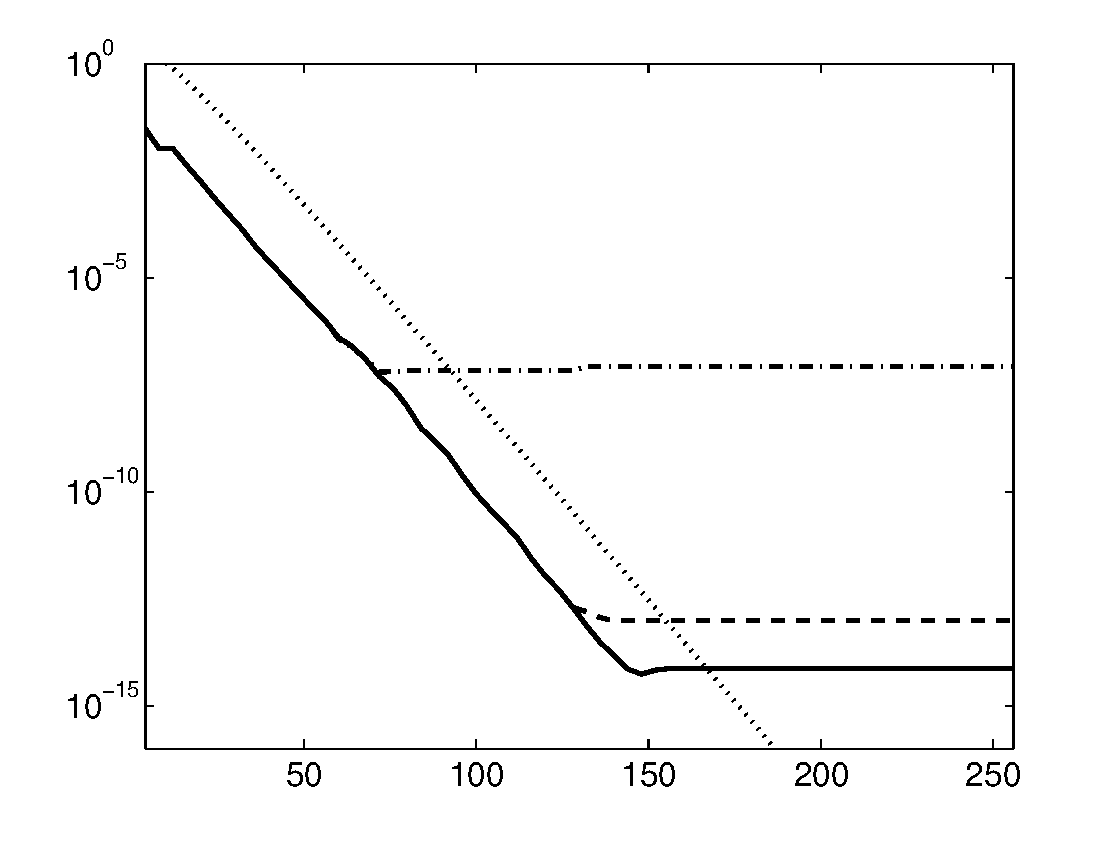
\includegraphics[width=0.45\textwidth]{images/poisson_test}}\hfill
  \subfigure[[The Singularity kernel $S_{h}$ for $h = 0.8$.]
  {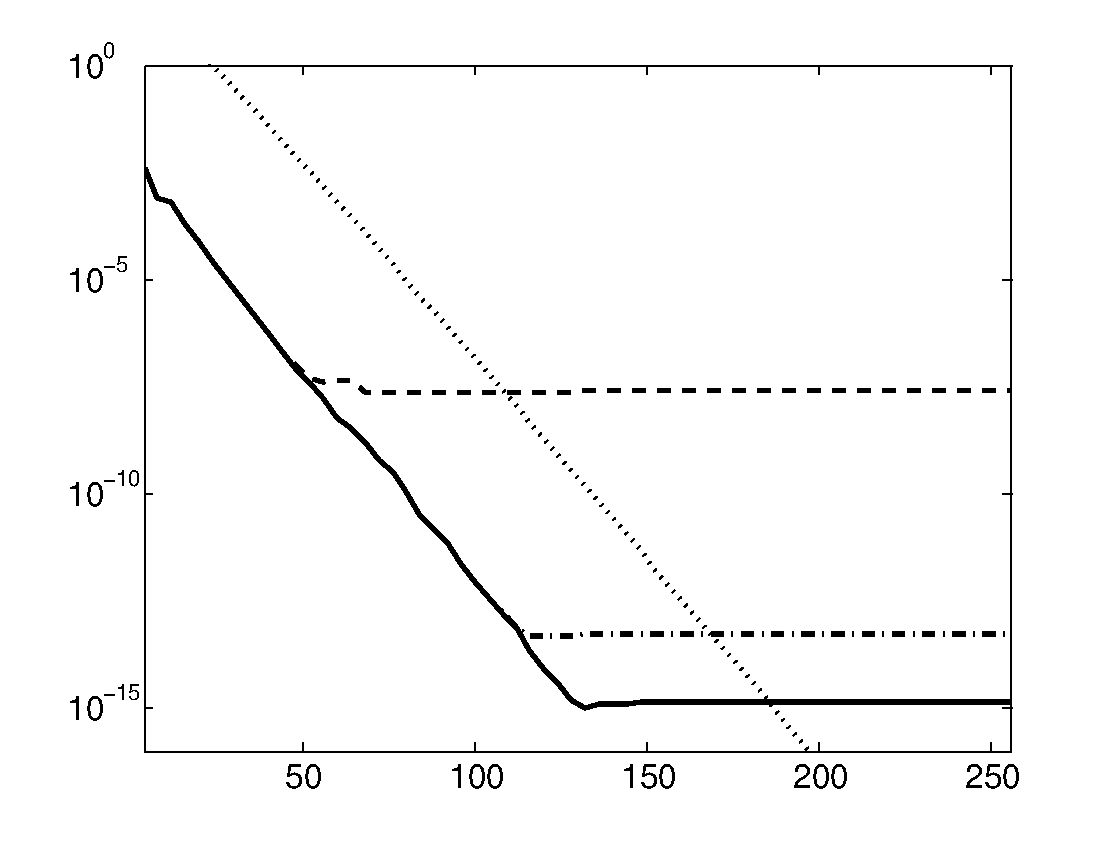
\includegraphics[width=0.45\textwidth]{images/singularity_test}}\\
  \caption{The error $E_{\infty}$ for $k = 4,8,\ldots,256$ and $L = D = 1000$: 
  Fast summation with NDSFT (solid), fast summation with NFSFT, 
  cut-off parameter $m = 3$ (dash-dot), fast summation with NFSFT, cut-off 
  parameter $m = 6$ (dashed), error estimate for 
  $E_{\infty}$ (dotted).}
  \label{fig:error}
\end{figure}
In Figure \ref{hTest},
we used in addition a second value $h=0.7$ for the locally supported 
kernel $L_{h,\lambda}$ in order to emphasize that the error 
bound is mainly dominated by the terms that depend on $\lambda$.
\begin{figure}[tb]
  \centering
  \subfigure[The locally supported kernel $L_{h,\lambda}$ for $h=0.3$, $\lambda = 7$. 
  The error estimate was fitted using $C_{\lambda} = 100$. For $C_{\lambda} = 50$ 
  the error estimate virtually coincides with the numerical result.]
  {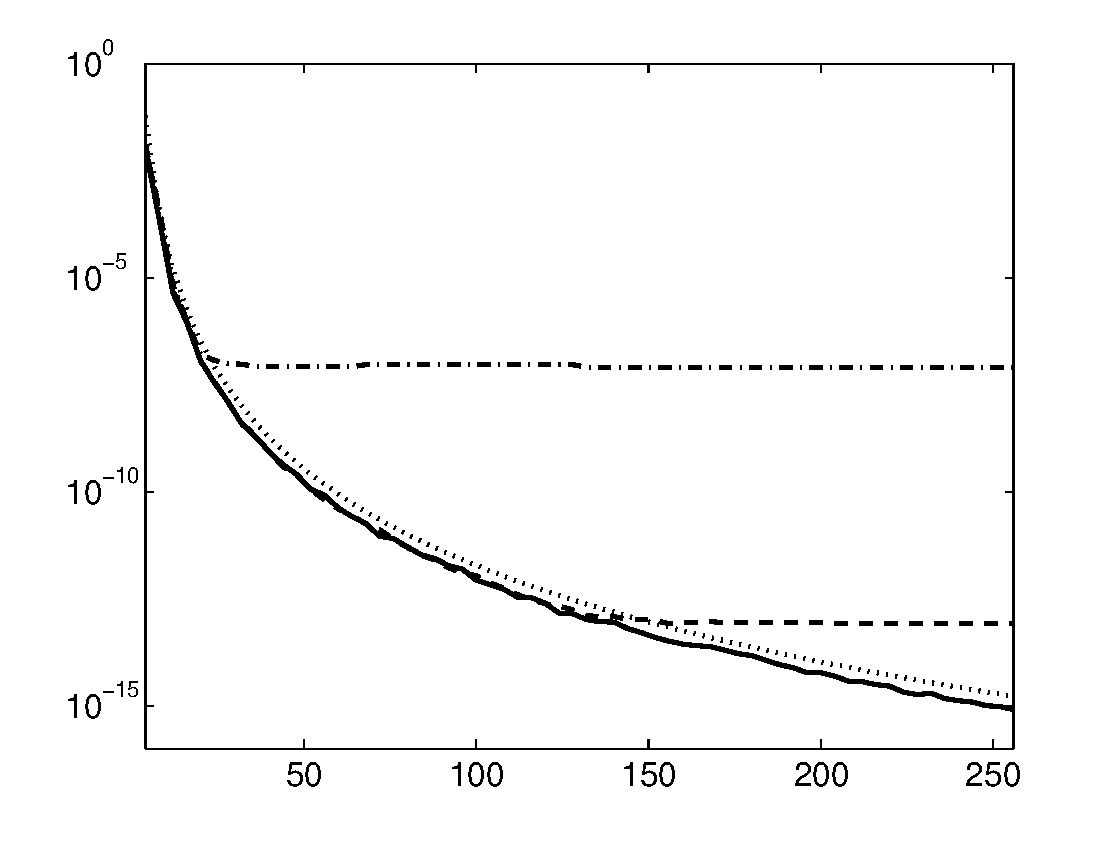
\includegraphics[width=0.45\textwidth]{images/locsupp_test}}\hfill
  \subfigure[The Gaussian kernel $G_{\sigma}$ for $\sigma=200$.]
  {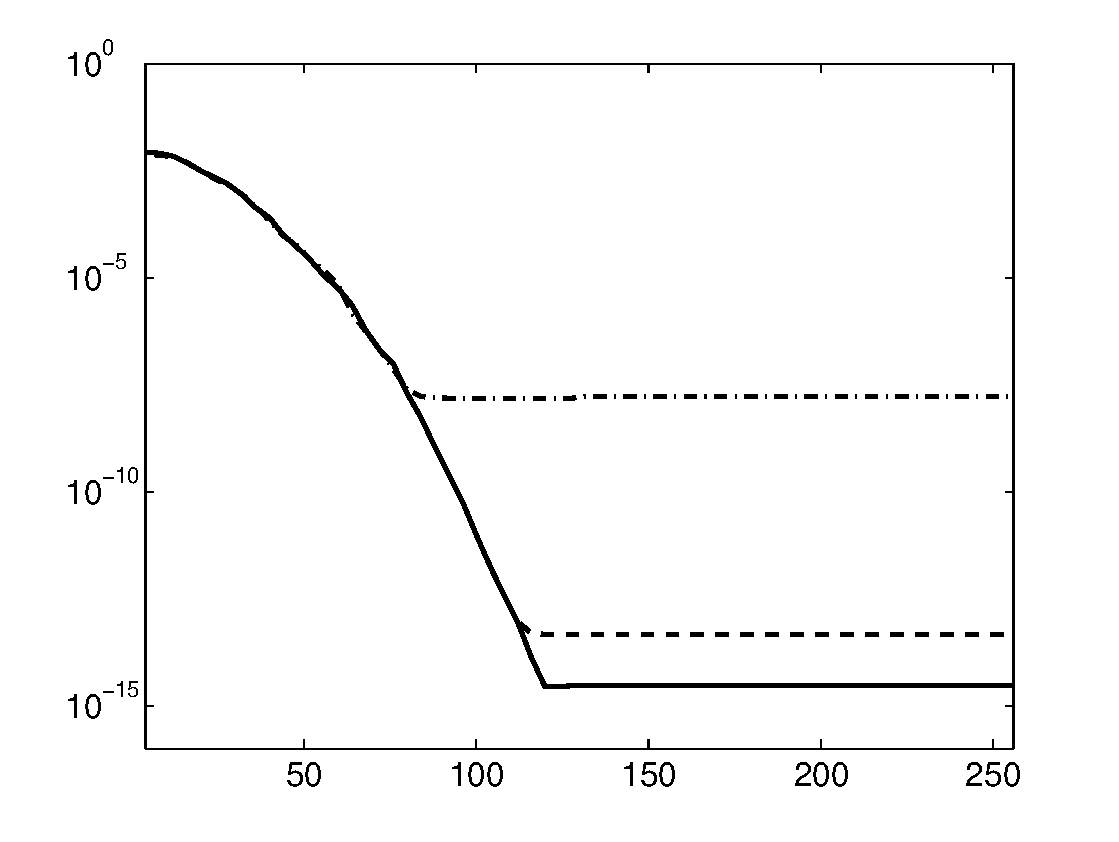
\includegraphics[width=0.45\textwidth]{images/gaussian_test}}
  \caption{The error $E_{\infty}$ for $k = 4,8,\ldots,256$ and $L = D = 1000$: 
  Fast summation with NDSFT (solid), fast summation with NFSFT, 
  cut-off parameter $m = 3$ (dash-dot), fast summation with NFSFT, cut-off 
  parameter $m = 6$ (dashed), error estimate for 
  $E_{\infty}$ (dotted).}
  \label{fig:error2}
\end{figure}

In order to 
demonstrate and isolate the specific influence of the threshold 
for the FLFT algorithm, we applied the fast summation algorithm 
to the Poisson kernel with the same parameters as in Figure 
\ref{SubFigurePoisson}, but with internally deactivated NFFT 
algorithm. Instead, we used the direct algorithm NDFT to 
evaluate the corresponding part. The result in Figure \ref{tTest}
shows that 
apparently, from a certain bandwidth $M$ on, a high threshold 
limits the accuracy of the
whole algorithm due to instable multiplication steps in the
FLFT algorithm. The situation even gets worse for increasing
$M$ as more and more instable steps are introduced into the 
cascade summation procedure.

\begin{figure}[tb]
  \centering
  \subfigure[The locally supported kernel $L_{h,\lambda}$ for $\lambda = 7$, and $h=0.3$ (solid),
  and $h=0.7$ (dashed). The error estimate (dotted) for $E_{\infty}$ was fitted 
  using $C_{\lambda} = 100$.]
  {
    \label{hTest}
    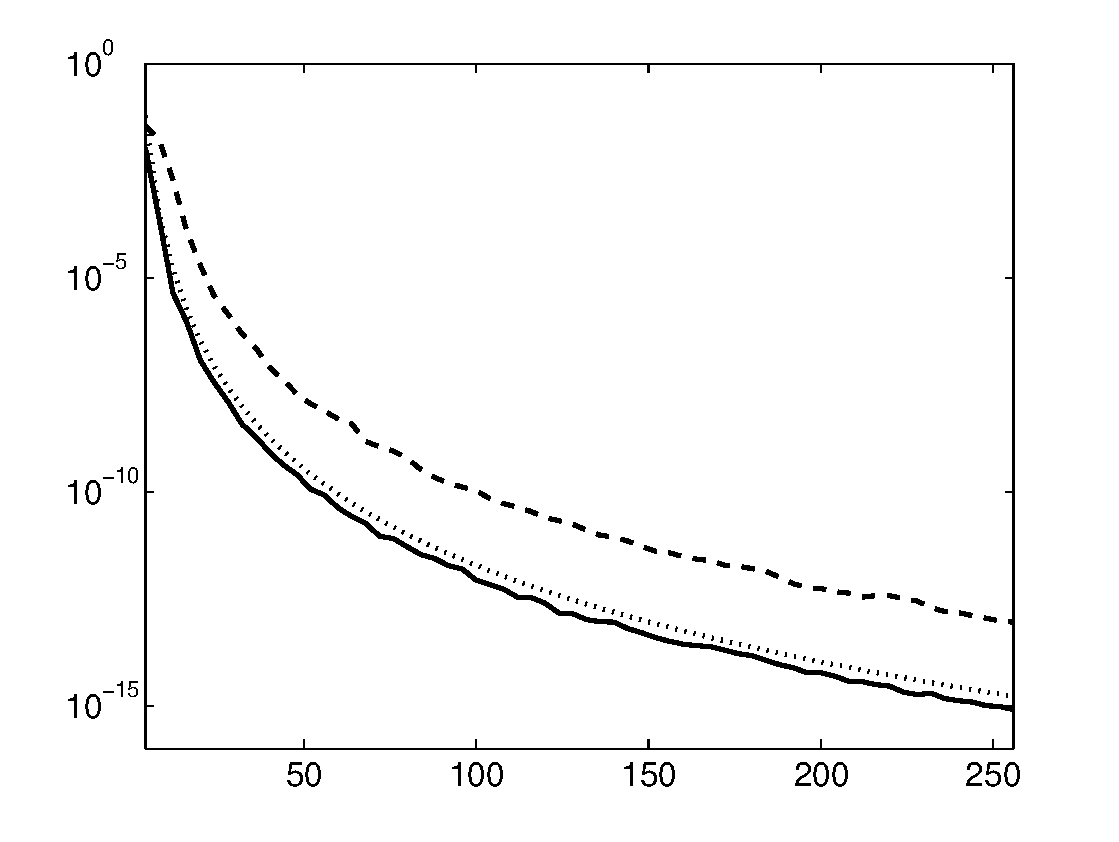
\includegraphics[width=0.45\textwidth]{images/locsup_h_test}}\hfill
  \subfigure[The Poisson kernel $Q_{h}$ for $h = 0.8$: Fast summation with 
  NFSFT/NDSFT and thresholds $10^6$ (solid), $10^9$ (dashed), $10^9$ (dash-dot). 
  The threshold steers the accuracy of the FLFT transformation.]
  {
    \label{tTest}
  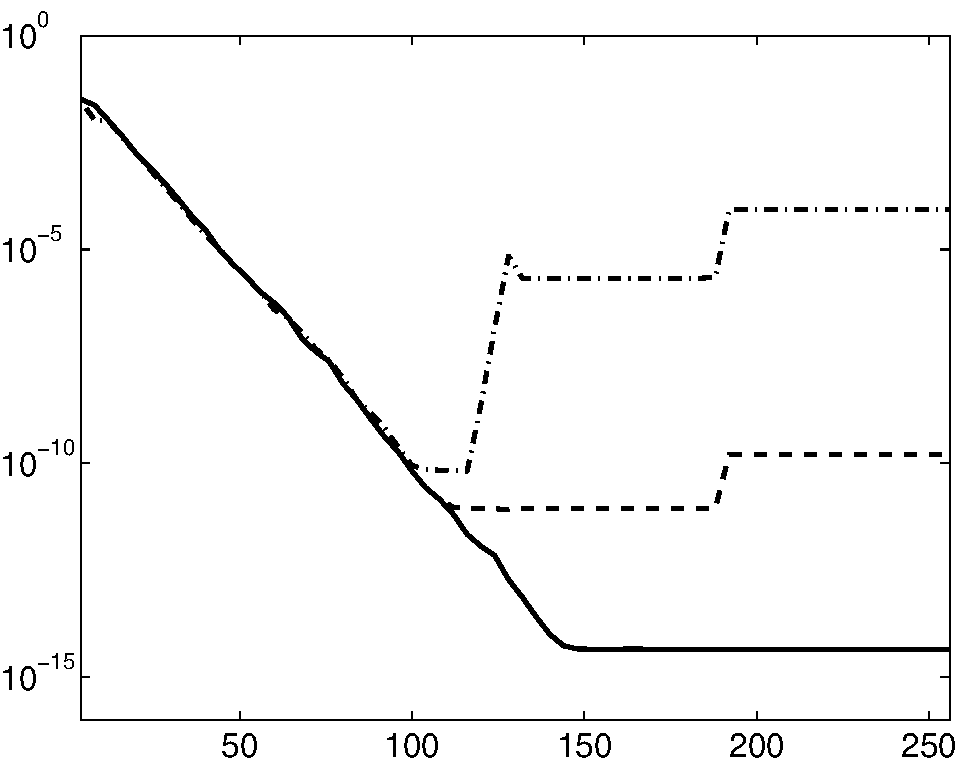
\includegraphics[width=0.45\textwidth]{images/threshold_test}}
  \caption{The error $E_{\infty}$ for $k = 4,8,\ldots,256$ and $L = D = 1000$.}
  \label{Figure:PoissonTest}
\end{figure}

Finally, we compare the computation time of the straightforward summation 
(direct algorithm), the straightforward summation with precomputed values 
$\fun{k}{\V{\eta}_{l} \cdot \V{\xi}_{d}}$, the fast summation algorithm (FS) 
with NDSFT, and the fast summation algorithm with NFSFT for increasing $L=D$.
The CPU time required by the four algorithms is shown in Table 
\ref{tab:TimeSpace}. As expected, the fast summation algorithms outperform the
straightforward algorithms for larger $L=D$, yielding $\bigo{D + L}$ 
algorithms. In addition, the NFSFT variant is considerably faster.

\begin{table}[ht!]
  \begin{center}
    \begin{tabular}{r|r|r|r|r|r}
        $L = D$ & direct alg. & w/precomp. & FS, NDSFT & FS, NFSFT & error $E_{\infty}$\\\hline
           $2^6$ & 1.0E-05 & 8.0E-05 & 1.1E-01 & 6.2E-01 & 7.7E-14\\
           $2^7$ & 6.0E-05 & 3.8E-04 & 2.2E-01 & 6.2E-01 & 6.5E-14\\
           $2^8$ & 2.5E-04 & 1.4E-03 & 4.5E-01 & 6.2E-01 & 4.1E-14\\
           $2^9$ & 1.0E-03 & 5.3E-03 & 8.9E-01 & 6.3E-01 & 2.8E-14\\
      $2^{10}$ & 4.0E-02 & 2.1E-02 & 1.8E+00 & 6.5E-01 & 3.6E-14\\
      $2^{11}$ & 1.6E+00 & 8.3E-02 & 3.6E+00 & 6.6E-01 & 1.8E-14\\
      $2^{12}$ & 6.4E+00 & 3.5E-01 & 7.1E+00 & 7.2E-01 & 1.3E-14\\
      $2^{13}$ & 2.6E+01 & 1.4E+00 & 1.4E+01 & 8.2E-01 & 6.7E-15\\
     $2^{14}$ & 1.0E+02 & -- & 2.8E+01 & 1.0E+00 & 5.5E-15\\
     $2^{15}$ & 4.1E+02 & -- & 5.7E+01 & 1.5E+00 & 4.0E-15\\
     $2^{16}$ & 1.6E+03 & -- & 1.1E+02 & 2.3E+00 & 2.9E-15\\
     $2^{17}$ & 6.6E+03 & -- & 2.3E+02 & 4.0E+00 & 2.4E-15\\
     $2^{18}$ & 2.6E+04 & -- & 4.6E+02 & 7.5E+00 & 1.9E-15\\
     $2^{19}$ & -- & -- & 9.1E+02 & 1.4E+01 & --\\
     $2^{20}$ & -- & -- & 1.8E+03 & 2.8E+01 & --\\
     $2^{21}$ & -- & -- & 3.6E+03 & 5.5E+01 & --\\
    \end{tabular}
  \end{center}
  \caption{CPU-Time and error $E_{\infty}$ for the fast summation algorithm.
    Note that we used averaged measurements in case of small times and the
    times/error $\paren{-}$ are not displayed due to the large response time or the 
    limited size of memory.}
  \label{tab:TimeSpace}
\end{table}


\section{Iterative Fourier Reconstruction}

As already mentioned, the matrix $\V{Y}$ is in general neither hermitian nor 
even square, but rectangular. For certain grids like $\mathcal{X^{\gl}}$ or 
$\mathcal{X^{\cc}}$, we derived inversion formula allowing for the computation 
of Fourier coefficients given function values on the corresponding grids 
based on quadrature formulae. 

In a more general approach, we like to compute Fourier coefficients 
$\paren{a_{k}^n}_{(k,n) \in \mathcal{I}^M}$ for a fixed bandwidth $M$
from function values $\paren{f_{d}}_{d=0}^D$ given on a sampling set
$\mathcal{X}$ with $D$ nodes, i.e. we like to compute a 'solution' to
\begin{equation}
  \label{Applications:Problem}
  \V{Y}_{\mathcal{X}} \V{a} \approx \V{f}.
\end{equation}

Now given an arbitrary sampling set $\mathcal{X}$ of $D$ nodes and a fixed 
bandwidth $M$, we consider two problems, i.e. the \emph{weighted linear 
least squares problem} and \emph{optimal interpolation}.

\subsection{Weighted Linear Least Squares Problem}
  For a comparatively low bandwidth, i.e. $(M+1)^2 \le D$, the matrix $\V{Y}$ 
  has more rows than columns and the system \eqref{Applications:Problem} is 
  overdetermined. We therefore consider the weighted linear least squares 
  problem
    \begin{equation}
      \label{Applications:Problem1}
      \norm{\V{f} - \V{Y}\:\V{a}}_{\V{W}}^2 \rightarrow \text{min},\ \V{W} = 
      \fun{\diag}{\paren{w_{d}}_{d=0}^{D-1}}, \ w_{d} \in \Rp.
    \end{equation}
  The diagonal matrix $\V{W}$ can be used to compensate for clustering of 
  the nodes. One might wish to weight the influence of nodes in sparsely 
  represented region more than in dense regions. 
  \begin{lemma}
    Problem \eqref{Applications:Problem1} is equivalent to the \emph{normal equation of the first kind}
    \begin{equation}
      \label{Applications:NormalEquation1}
      \V{Y^{\h}} \; \V{W} \; \V{Y} \V{a} = \V{Y^{\h}} \; \V{W} \; \V{f}.
    \end{equation}
  \end{lemma}
  \begin{proof}
    By definition, minimizing $\norm{\V{f} - \V{Y}\:\V{a}}_{\V{W}}^2 = 
    \norm{\V{W}^{1/2}\paren{\V{f} - \V{Y}\:\V{a}}}_2^2$ yields
    \[
      \fun{F}{\V{a}} := \V{a}^{\h} \; \V{Y}^{\h} \; \V{W} \; \V{Y} \; \V{a} - 
      2 \; \V{a}^{\h} \; \V{Y}^{\h} \; \V{W} \; \V{f} +  \V{f}^{\h} \; 
      \V{W} \; \V{f} \rightarrow \text{min}.
    \]
    The quadratic functional $F$ is convex, since 
    $\V{Y}^{\h} \; \V{W} \; \V{Y}$ is symmetric positive semi-definite 
    (positive definite if $\V{Y}$ has full rank) and the necessary condition 
    for minimizing $F$ requires $\V{a}$ to obey 
    $\triangledown \fun{f}{\V{a}}^T = \V{0}$, or equivalently
    \[
      \V{Y^{\h}} \; \V{W} \; \V{Y} \V{a} = \V{Y^{\h}} \; \V{W} \; \V{f}.
    \]
  \end{proof}
  The theoretical and numerical treatment of Problem \eqref{Applications:Problem1}
  has been studied extensively (see for example \cite{bjoerk}). Generally, one tries to
  avoid normal equations since they are often subject to numerical instabilities. In
  our setting, however, computing a solution to \eqref{Applications:Problem1}
  by means of the QR-decomposition or SVD is no practical way, due to performance and 
  memory requirements. But the Algorithms \ref{} (NFSFT) and \ref{} (adjoint NFSFT)
  derived in Section \ref{NFSFT} allow for an application of numerical methods to
  \eqref{Applications:NormalEquation1}. A well know algorithm is the 
  \emph{conjugate gradient method (CG)} modified for 
  \eqref{Applications:NormalEquation1} and denoted as \emph{CGNR}, where N stands 
  for ''Normal'' and R for ''Residual''. Other, simpler methods we won't mention here
  include the \emph{steepest descent} method and the \emph{Landweber iteration}. We 
  refer to \cite{bjoerk} and \cite{golo} for details. The CGNR algorithm is summarized in 
  Algorithm \ref{Applications:Algorithm:CGNR}. We notice that the algorithm does not 
  need to store the matrices $\V{Y}$, $\V{Y}^{\h}$ or even $\V{Y}^{\h} \; \V{W} \; 
  V{Y}^{\h}$ explicitly. Instead, we only need to perform multiplications with 
  $\V{Y}$ and $\V{Y}^{\h}$ which corresponds to applications of Algorithms 
  \ref{} and \ref{}, respectively.
 
  \begin{algorithm}[tb]
    \caption{CGNR}
    \label{Applications:Algorithm:CGNR}    
	  \begin{algorithmic}
	    \STATE  Input:  $\V{f} \in \C^{D}$, $\V{a}_{0} \in C^{(M+1)^2}$
	    \STATE
	    \STATE $\V{r_{0}} := \V{f} - \V{Y} \; \V{a}_{0}$
	    \STATE $\V{z_{0}} := \V{Y}^{\h} \; \V{W} \V{r}_{0}$
	    \STATE $\V{p_{0}} := \V{z}_{0}$
	    \STATE 
	    \FOR {$l=0,\ldots,\text{until convergence}$} 
	      \STATE $\V{v}_{l} := \V{Y} \; \V{p}_{l}$
	      \STATE $\alpha_{l} := \frac{\norm{\V{z}_{l}}_{2}^2}{\norm{\V{v}_{l}}_{2}^2}$  
	      \STATE $\V{a}_{l+1} := \V{a}_{l} + \alpha_{l} \V{p}_{l}$
	      \STATE $\V{r}_{l+1} := \V{r}_{l} - \alpha_{l} \V{w}_{l}$
	      \STATE $\V{z}_{l+1} := \V{Y}^{\h} \; \V{r}_{l+1}$
	      \STATE $\beta_{l}   := \frac{\norm{\V{z}_{l+1}}_{2}^2}{\norm{\V{z}_{l}}_{2}^2}$
	      \STATE $\V{p}_{l+1} := \V{z}_{l+1} + \beta_{l} \V{p}_{l}$
	    \ENDFOR
	    \STATE
	    \STATE Output: $\V{a}_{l}$ where $l$ is the iteration after which the loop has terminated.
	  \end{algorithmic}
  \end{algorithm}
  
  \begin{example}
    We considered the NASA GSFC and NIMA Joint Geopotential Model, \emph{EGM96} (see 
    \verb+http://cddis.gsfc.nasa.gov/926/egm96/egm96.html+) and the corresponding model 
    dataset consisting of Fourier coefficients $\paren{a_{k}^n}_{(k,n) \in \mathcal{I}^M}$
    for $M$ up to 360.
    The corresponding function $f$ was evaluated on the Clenshaw-Curtis grid 
    $\mathcal{X}^{\cc}$ corresponding to $M = 360$ and consisting of $2(M+1)(2M+1) = 520,562$
    nodes. Algorithm \ref{Applications:Algorithm:CGNR} was applied with the corresponding 
    weight matrix $\V{W}^{\cc}$ and an initial guess $\V{a}_{0} = \V{0}$. In theory, the
    algorithm terminates after one step with the original Fourier vector
  \end{example}
  
  
  
%  \begin{remark}
%    For the NFFT, Fourier reconstruction methods have been investigated for example by \cite. 
%    We follow the lines in \cite for our setup. However, theoretical results leading to 
%    stability results have still to be  developed.
%  \end{remark}
    
    
\begin{figure}[tb]
  \centering
  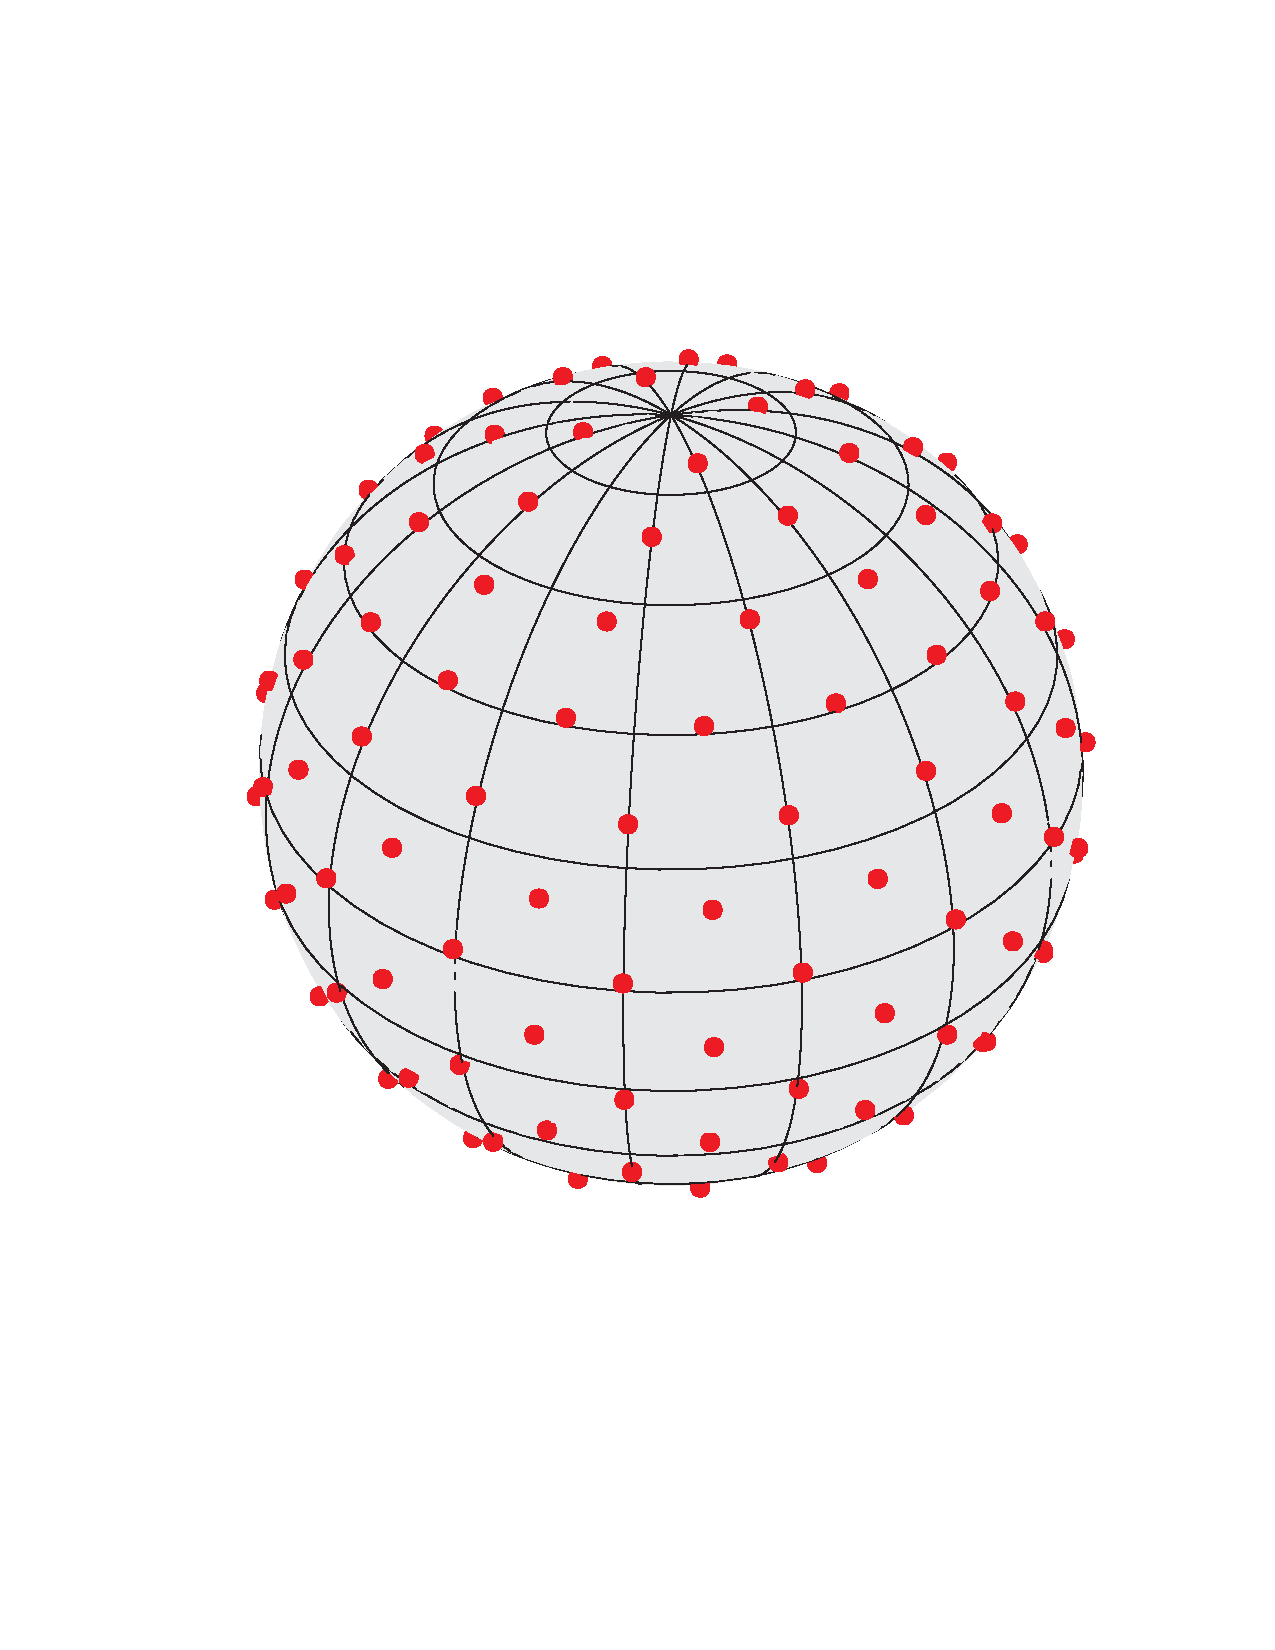
\includegraphics[width=12cm]{images/healpix}
  \caption{To be written...}
  \label{healpix}
\end{figure}


